\section{Sincronizzazione tra processi}
Abbiamo principalmente questi tipi di interazione tra processi:
\begin{itemize}
    \item cooperazione: sincronizzazione diretta o esplicita, quando è richiesta dall' utente.
    Per esempio nello scambio di messaggi.

    \item competizione: sincronizzazione indiretta o implicita, quando è chiesta dal SO.
    Per esempio nell' accesso ad una risorsa.
    
    \item interferenza: una situazione di errore che voglio evitare.
    Per esempio in un buffer condiviso tra più processi, se prima devo scrivere e poi leggere, mai scrivere due volte di fila o mai leggere due volte di fila, non rispettando queste regole perdo l' integrità della comunicazione.
\end{itemize}

\subsection{Tipi di comunicazione}
\subsubsection{Interazione a memoria comune}
\begin{figure}[H]
    \centering
    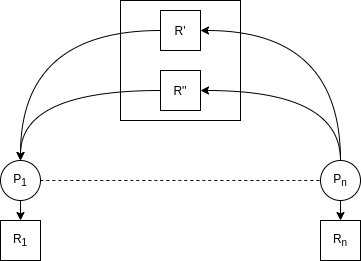
\includegraphics[width=250px]{images/6_Sincronizzazione_tra_processi/memoria_comune.png}
\end{figure}
L' accesso a $R'$ e $R''$ deve essere in mutua esclusione, quelli a $R_1$ e $R_n$ no perché sono private ed accessibili solo al processo che le detiene.

\subsubsection{Interazione a memoria locale/scambio di messaggi}
\begin{figure}[H]
    \centering
    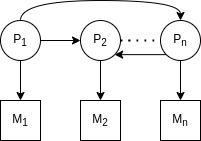
\includegraphics[width=175px]{images/6_Sincronizzazione_tra_processi/scambio_di_messaggi.png}
\end{figure}
Lo scambio dei messaggi è gestito dal sistema operativo, prima di usare i dati vanno quindi copiati nella memoria locale del processo.
Questo meccanismo è indispensabile nei sistemi a memoria distribuita fisicamente, ad esempio i sistemi MIMD a memoria distribuita.

NB: nelle macchine MIMD-SM si dovrà solo copiare da una memoria all' altra e non si hanno veri e propri messaggi.

Usano gli stessi sistemi usati nelle reti per scambiarsi i messaggi creando di fatto una astrazione di connessione punto-punto.
Lo scambio di messaggi si può fare anche su macchine SISD, quindi tutto sullo stesso calcolatore. E' possibile distribuire il carico su diversi calcolatori o centralizzare il tutto, senza cambiare implementazione.

\subsection{Mutua esclusione}
Nei sistemi a memoria condivisa bisogna garantire l' accesso in mutua esclusione alla memoria.
Es:
\begin{verbatim}
    T stack[n]
    int top = -1
    
    T prelievo(){
        T temp
        temp = stack[top]
        top++
        return temp
    }
    
    void inserimento(T y){
        top++
        stack[top] = y
    }
\end{verbatim}

Poniamo il caso di avere due processi che utilizzino entrambi questa struttura condivisa: $P_1$ e $P_2$, se li lancio in parallelo potrebbe accadere:
\begin{itemize}
    \item $t_0$ - $P_1$
    \begin{verbatim}
        top++
    \end{verbatim}
    porto il puntatore ad un elemento vuoto dello stack

    \item $t_1$ - $P_2$
    \begin{verbatim}
        temp = stack[top]
    \end{verbatim}
    copio un elemento indefinito

    \item $t_2$ - $P_2$
    \begin{verbatim}
        top--
    \end{verbatim}
    torno all' ultimo elemento vero
    
    \item $t_3$ - $P_1$
    \begin{verbatim}
        stack[top] = y
    \end{verbatim}
    scrivo il nuovo valore sull' ultimo elemento
\end{itemize}
Abbiamo ottenuto una struttura \emph{inconsistente}!

Possiamo definire queste funzioni come \emph{sezioni critiche}, sono le sezioni del codice che accedono alla struttura condivisa.
L' inconsistenza c'è perché le istruzioni non sono state eseguite in maniera atomica!
Se avessi avuto l' atomicità le operazioni sarebbero andate bene in qualsiasi ordine, avrei avuto due strutture diverse ma non importa l'ordine in quanto la richiesta è di prendere l' elemento al top dello stack in quel momento, indipendentemente da quale elemento esso sia.

\subsubsection{Soluzione 1 - sbagliata}
Possiamo pensare ad una soluzione del tipo: creo una variabile condivisa \emph{occupato} che indica:
\begin{itemize}
    \item 1: risorsa occupata
    \item 0: risorsa libera
\end{itemize}
Scrivo dunque un codice del genere:

\begin{verbatim}
P1:
    while(occupato)
    occupato = 1
    < sezione critica A >
    occupato = 0
    
P2:    
    while(occupato)
    occupato = 1
    < sezione critica B >
    occupato = 0
\end{verbatim}
Abbiamo creato un protocollo facile da rispettare ed uguale per tutti!
\emph{Tuttavia è sbagliato!}

Se a $t_0$ $P_1$ esegue il while, trova 0, lo scheduler switcha a $P_2$, esegue il while, trova 0 abbiamo entrambi i processi nella sezione critica allo stesso momento!
Questo potrebbe succedere in quanto il prologo non è atomico, infatti abbiamo che \emph{occupato} è una risorsa condivisa quindi anche lei va gestita in mutua esclusione.
Inoltre è da notare che il processo in attesa spreca il suo tempo all' interno di una \emph{busy wait}.

\subsubsection{Soluzione con test-and-set}
Alcuni processori mettono a disposizione istruzioni dette \emph{test-and-set} cioè nella stessa istruzione si occupano di leggere un valore e settarlo ad un altro, il tutto in maniera atomica.
Andremo quindi a scrivere:
\begin{verbatim}
    lock(x):
        TSL registro, x
            ; copio x nel registro
            ; e pongo x ad 1
        CMP registro, 0
        JNE lock
            ; se x era != 0 torno a lock
        RET
        
    unlock(x):
        MOV x, 0
            ; metto x a 0
        RET
\end{verbatim}
TSL dunque è atomica per definizione!
Se $x$ è 0, quindi libera, la setta e diventa il detentore della risorsa uscendo dal ciclo, se $x$ è 1, quindi occupata, la setta sempre ad 1 e continua il ciclo senza intaccare la coerenza del valore.
TSL ci permette di avere l' atomicità in quanto locka il bus per eseguire la sua lettura e la sua scrittura, quindi è corretta anche su sistemi multi-processore.

Posso quindi scrivere il codice nella forma:
\begin{verbatim}
P1:
    lock(x)
    < sezione critica A >
    unlock(x)

P2:    
    lock(x)
    < sezione critica B >
    unlock(x)
\end{verbatim}
Questa soluzione ci garantisce una mutua esclusione, funzionamento nei sistemi multi-processore ma comunque mantiene le attese attive e pertanto conviene usarla quando la sezione critica è molto piccola, per minimizzare appunto l'attesa.

\subsection{Semaforo}
E' una struttura dati con un valore intero ed una coda di processi:
\begin{verbatim}
    wait(s):
        if s.value == 0:
            < sospendo il processo e lo metto in coda >
        else:
            s.value = s.value - 1

    signal(s):
        if c'è qualcosa in coda:
            estraggo dalla coda e metto in esecuzione
        else:
            s.value = s.value + 1
\end{verbatim}
Queste operazioni vanno eseguite in maniera atomica, quindi devono essere primitive di sistema e devono essere eseguite con le interruzioni disabilitate.
Su più processori potrei usare le primitive lock-unlock come prologo!
Siccome è il sistema a gestire tutto quanto ho overhead minore e posso eliminare le attese attive.

Se value è inizializzato ad un certo valore $n$ saranno $n$ i processi a poter passare la wait prima di essere sospesi.

\subsubsection{Mutex}
Posso quindi usare un semaforo per creare la struttura \emph{mutex} per risolvere definitivamente il problema della mutua esclusione:
\begin{verbatim}
    wait(mutex)
    < sezione critica >
    signal(mutex)
\end{verbatim}
questa è una procedura che deve essere eseguita per ogni sezione critica, l' onere è sul programmatore! 

\subsection{Produttore-consumatore}
Un processo produttore deposita un messaggio in un buffer, il processo consumatore preleva il messaggio dal buffer, nel modello a memoria condivisa abbiamo questa situazione:
\begin{figure}[H]
    \centering
    
\includegraphics[width=200px]{images/6_Sincronizzazione_tra_processi/produttore-consumatore.png}
\end{figure}
abbiamo le seguenti regole:
\begin{itemize}
    \item il produttore non deve inserire un messaggio nel buffer se questo è pieno
    \item il consumatore non deve prelevare un messaggio dal buffer se questo è vuoto
    \item al buffer bisogna accederci in mutua esclusione
\end{itemize}
Usiamo due semafori:
\begin{itemize}
    \item \emph{spazio\_disponibile}: indica se il buffer è libero, è inizializzato ad 1
    \item \emph{messaggio\_disponibile}: indica se c'è un nuovo messaggio, è inizializzato a 0
\end{itemize}
\begin{verbatim}
    Produttore:
    do{
        < produco il messaggio >
        wait(spazio_disponibile)
            // aspetto che ci sia spazio disponibile
        < deposito il messaggio >
        signal(messaggio_disponibile)
            // segnalo che c'è un nuovo messaggio
    }while(!fine)
    
    Consumatore:
    do{
        wait(messaggio_disponibile)
            // aspetto che ci sia un nuovo messaggio
        < prelevo il messaggio >
        signal(spazio_disponibile)
            // segnalo di averlo preso
        < consumo il messaggio >
    }while(!fine)
\end{verbatim}

\subsection{Bounded buffer problem - N produttori, 1 consumatore}
E' una variante del problema produttore-consumatore in cui abbiamo $N$ produttori ed 1 solo consumatore.
Possiamo pensare di inizializzare la variabile \emph{spazio\_disponibile} ad $N$ in modo da accogliere più processi produttori assieme, tuttavia se non modifico la soluzione precedente, avendo $N$ produttori che entrano allo stesso tempo non garantisco l' accesso in mutua esclusione alla struttura dati!

Per risolvere devo pertanto inserire un nuovo semaforo \emph{mutex} per gestire questo accesso:
\begin{verbatim}
    Produttore:
    do{
        wait(spazio_disponibile)
            // aspetto che ci sia spazio disponibile
        wait(mutex)
            // aspetto di poter accedere alla struttura
        < deposito il messaggio >
        signal(mutex)
            // rilascio la struttura
        signal(messaggio_disponibile)
            // segnalo di aver inserito un nuovo messaggio
    }while(!fine)
    
    Consumatore:
    do{
        wait(messaggio_disponibile)
            // aspetto che ci sia un nuovo messaggio
        wait(mutex)
            // aspetto di poter accedere alla struttura
        < prelevo il messaggio >
        signal(mutex)
            // rilascio la struttura
        signal(spazio_disponibile)
            // segnalo di averlo preso
        < consumo il messaggio > 
    }while(!fine)
\end{verbatim}

Si noti che se invertissi le wait tra \emph{mutex} e \emph{messaggio\_disponibile} potrei ricadere in \emph{deadlock} in quanto:
\begin{verbatim}
    wait(mutex)
    wait(spazio_disponibile)

    wait(mutex)
    wait(messaggio_disponibile)
\end{verbatim}

\begin{itemize}
    \item buffer pieno, un produttore prova ad entrare ed acquisice l' accesso in mutua esclusione sulla struttura, tuttavia rimane bloccato alla richiesta sullo spazio disponibile. In parallelo arriva un consumatore che potrebbe sbloccarlo, ma non può accedere alla risorsa perché il mutex è occupato e quindi si mette in pausa.
    
    \item buffer vuoto, un consumatore prova ad entrare ed acquisisce l' accesso in mutua esclusione, rimane bloccato in quanto la struttura è vuota. In parallelo arriva un produttore che vorrebbe inserire un messaggio ma non può perché la risorsa è occupata.
\end{itemize}
NB: non bloccare le risorse se non le puoi utilizzare!

\subsection{Readers \& writers}
Immaginiamo di avere un dataset condiviso tra più processi concorrenti:
\begin{itemize}
    \item lettore: legge e basta, non modifica niente
    \item scrittore: può sia leggere che scrivere
\end{itemize}
si vuole permettere a più lettori di leggere in contemporanea ma di scrivere a solo uno scrittore per volta.
Inoltre vogliamo che: se ci sono lettori non possano entrare scrittori e se c'è uno scrittore non possano entrare lettori.
Usiamo queste 3 strutture:
\begin{itemize}
    \item \emph{readcount}: variabile intera che ci dice quanti lettori ci sono al momento
    \item \emph{mutex\_readcount}: per gestire l' accesso concorrente alla variabile readcount
    \item \emph{mutex\_writers}: mutex per l'accesso esclusivo in scrittura
\end{itemize}
proponiamo la seguente soluzione:
\begin{verbatim}
    Writer:
        wait(mutex_writers)
            // aspetto di poter accedere alla struttura
        < scrivo >
        signal(mutex_writers)
            // libero la struttura

    Reader:
        wait(mutex_readcount)
            // aspetto l'accesso a readcount
        readcount++
            // incremento il conteggio lettori
        if (readcount == 1):
            wait(mutex_writers)
            // se sono il primo lettore aspetto
            // che non ci siano scrittori
            // sulla struttura e ne prendo il controllo
        signal(mutex_readcount)
            // rilascio readcount
        
        < leggo >
        
        wait(mutex_readcount)
            // aspetto l'accesso a readcount
        readcount--
            // un lettore in meno
        if (readcount == 0):
            signal(mutex_writers)
            // se sono l'ultimo lettore
            // permetto l'accesso ad uno scrittore
        signal(mutex_readcount)
\end{verbatim}

\subsection{Readers \& writers con priorità}
Facciamo una variazione al problema precedente: appena uno scrittore è pronto, scrive il prima possibile cioè lo scrittore ha la precedenza sui lettori.

\begin{verbatim}
    BOH, DEVO FARLO PRIMA O POI
\end{verbatim}
NB: avendo introdotto le priorità si rischia la starvation dei lettori.

\subsection{Dining philosophers - 5 filosofi}
Abbiamo 5 filosofi a cena che devono mangiare ed abbiamo 5 bacchette ognuna delle quali posizionate tra l' uno e l' altro.
Per mangiare devono prendere 2 bacchette, una per volta.
Una volta che uno ha mangiato rilascia entrambe le bacchette.
\begin{figure}[H]
    \centering
    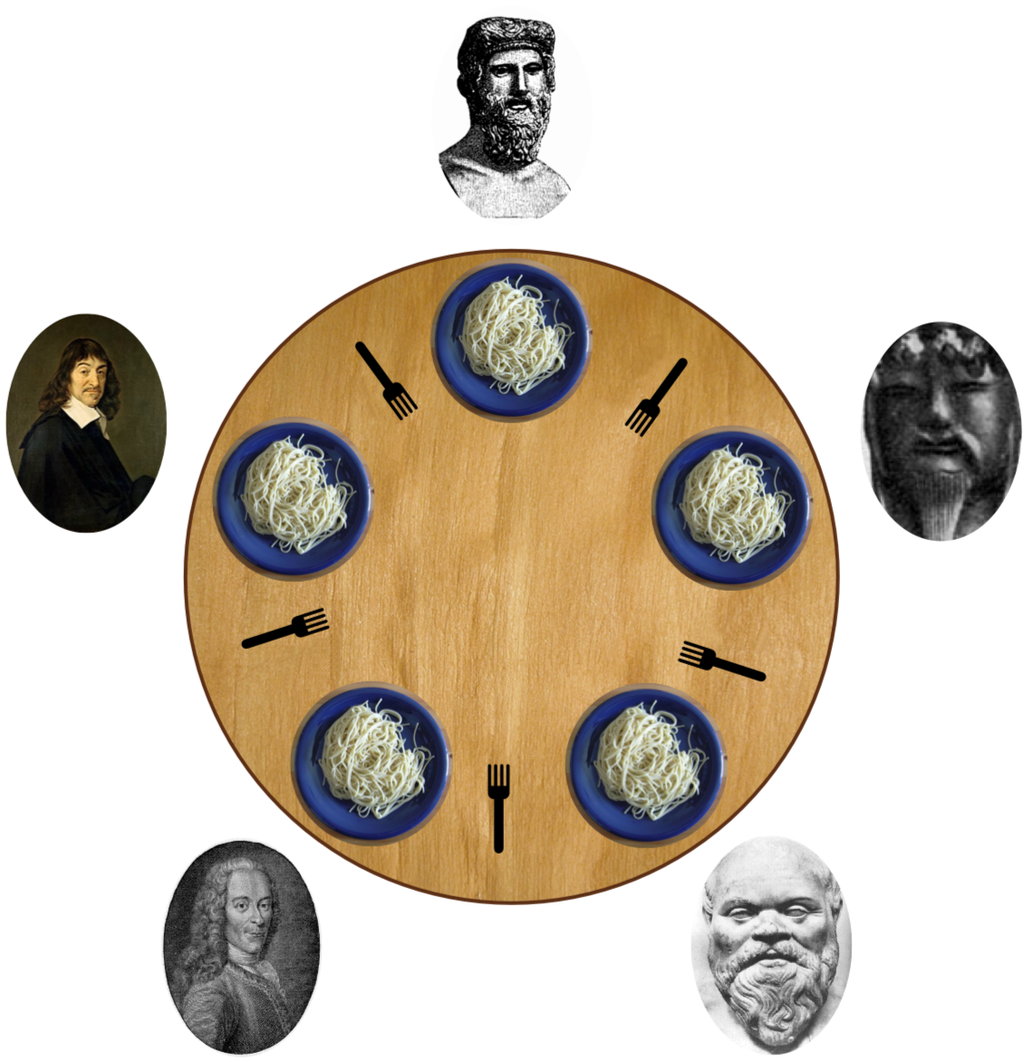
\includegraphics[width=200px]{images/6_Sincronizzazione_tra_processi/dining_philosophers_problem.png}
\end{figure}
Visto in maniera più pratica abbiamo 5 processi che vogliono accedere a delle risorse e possono trovarsi in 3 stati:
\begin{itemize}
    \item \emph{pensante}: non consuma risorse
    \item \emph{affamato}: è in cerca di risorse 
    \item \emph{mangiante}: ha le risorse e le sta consumando
\end{itemize}
Si vuole un solo codice che funzioni per tutti i filosofi e che sia conforme a questo protocollo:
\begin{itemize}
    \item prima mi procuro la bacchetta destra
    \item poi mi procuro la bacchetta sinistra
    \item mangio
    \item rilascio la bacchetta destra
    \item rilascio la bacchetta sinistra
\end{itemize}
Proponiamo la seguente soluzione usando un array di mutex sulle bacchette:
\begin{verbatim}
    do{
        wait(chopstick[i])
        wait(chopstick[(i + 1) % 5])
            // eat
        signal(chopstick[i])
        signal(chopstick[(i + 1) % 5])
    }while(!fine)
\end{verbatim}
Tuttavia questa soluzione NON funziona!
Supponiamo che il primo filosofo prenda la bacchetta alla sua destra, successivamente il secondo prende la bacchetta alla sua destra, e così via.
Alla fine del giro abbiamo che ogni filosofo ha la sua bacchetta destra ma è in attesa che si liberi la sinistra.
Ci troviamo in una \emph{attesa ciclica}.

\subsection{Monitor}
Costruiamo una astrazione ad alto livello chiamata \emph{monitor} per fornire meccanismi di sincronizzazione.
E' una struttura dati astratta così composta:
\begin{verbatim}
    monitor{
        //shared variables
        
        procedure P1(...){...}
        procedure P2(...){...}
        ...
        procedure Pn(...){...}

        init(...){...}
    }
\end{verbatim}
Solo un processo per volta può essere attivo all' interno del monitor e solo le procedure interne possono accedere alle variabili interne.

Introduciamo all' interno del monitor le \emph{variabili condizionali}.
Su queste variabili si può solo fare:
\begin{itemize}
    \item wait: il processo che la invoca si stoppa sempre e si mette in coda sulla variabile
    \item signal: se c'è una coda sulla variabile si prende il primo processo e lo si riattiva, altrimenti non fa niente
\end{itemize}
Le signal sulle variabili condizionali può seguire due politiche:
\begin{itemize}
    \item \emph{signal and wait}: alla signal sospendo il processo che la esegue finché il processo in wait non termina o si stoppa
    \item \emph{signal and continue}: alla signal il processo che la esegue continua fino ad uscire o alla prossima wait
\end{itemize}

\subsubsection{Soluzione al problema dei 5 filosofi}
Possiamo usare i monitor per risolvere il problema dei 5 filosofi:
\begin{verbatim}
    monitor DiningPhilosophers {
        enum { THINKING, HUNGRY, EATING) state [5];
        condition self [5];

        void pickup (int i) {
            state[i] = HUNGRY;
            test(i);
            if (state[i] != EATING) self [i].wait;
        }

        void putdown (int i) {
            state[i] = THINKING;
            // test left and right neighbors
            test((i + 4) % 5);
            test((i + 1) % 5);
        }

        void test (int i) {
            if ((state[(i+4) % 5] != EATING) &&
                (state[i] == HUNGRY) &&
                (state[(i+1) % 5] != EATING)) {
                    state[i] = EATING;
                    self[i].signal();
            }
        }

        initialization_code() {
            for (int i = 0; i < 5; i++)
                state[i] = THINKING;
        }
    }
\end{verbatim}
Partiamo dalla logica che se un filosofo è affamato può passare allo stato mangiante solo se i suoi vicini non stanno già mangiando, come variabili normali ho un vettore di stati a rappresentare lo stato dei 5 filosofi, dopodiché implemento una funzione di controllo \emph{test} che mi dice se i miei vicini stanno mangiando, se i miei vicini non stanno mangiando ed io sono affamato mi porto nello stato mangiante.

Successivamente devo implementare le funzioni di utilità del monitor: in questo caso la \emph{pickup} e la \emph{putdown}.
La funzione \emph{pickup} deve controllare di poter mangiare quindi si porta nello stato affamato, esegue il test e se il test ha esito negativo si porta in attesa sulla risorsa \emph{i}.
Nella funzione \emph{putdown} invece torno allo stato pensante liberando le risorse prese e lascio ai miei vicini la possibilità di transitare verso lo stato mangiante se dovessero essere affamati; per fare ciò eseguo la funzione di test sui miei vicini, oltre al test la funzione esegue anche una signal sulla risorsa \emph{i} sulla quale faccio il test. 

Di fatto nella pickup mi metto in attesa se non posso acquisire le risorse e mi farò risvegliare dalla putdown di uno dei due vicini.

Nel monitor posso avere più processi che eseguono la pickup:
\begin{itemize}
    \item il primo che riesce si ritrova mangiante ed abbandona il monitor, non eseguendo alcuna wait, entrando nella sua sezione critica
    \item quando un suo vicino eseguirà una pickup si metterà in attesa sulla variabile condizionale
    \item quando il primo eseguirà una putdown rilascerà le risorse prese e risveglierà i vicini se sono in pausa
\end{itemize}

Dal lato applicazione il codice apparirà così:
\begin{verbatim}
    DiningPhilosophers.pickup(i)
        // sezione critica
    DiningPhilosophers.putdown(i)
\end{verbatim}

In questa soluzione non abbiamo deadlock in quanto è garantita la mutua esclusione tra i processi, le conditions implementate per avere sempre una wait ci evitano le attese cicliche.
La starvation è ancora possibile, cioè: qualche filosofo potrebbe ritardare per molto tempo o subire un blocco permanente, questo succede perché ogni filosofo controlla al massimo i suoi vicini quindi se ci sono tanti eventi che riguardano lo stesso filosofo sarà interessato solo un gruppo ristretto. 

\subsubsection{Implementazione di un monitor}
Uno dei punti a favore del monitor è che spesso l' implementazione è già data in un qualche linguaggio di programmazione o in qualche framework, questo libera il programmatore dalla necessità di dover implementare queste strutture critiche da se.
Implementiamo di seguito un monitor usando la politica signal \& wait per le variabili conditions:
\begin{verbatim}
    // variabili del monitor
    semaphore mutex
        // ci regola l'accesso in mutua 
        // esclusione al monitor
    semaphore next
        // ci fornisce la coda dei
        // processi in entrata nel monitor
    int next_count = 0
        // mantiene la lunghezza della
        // coda in entrata

        // codice della procedura
        // generica nel monitor
    function Fi():
        wait(mutex)

            F()

            // se ci sono processi in coda
            // già dentro il monitor
            // lascio loro la precedenza
        if(next_count > 0)
            signal(next)
        else:
            // altrimenti ne faccio entrare
            // un altro dall' esterno
            signal(mutex)
\end{verbatim}
Possiamo vedere questa implementazione come un passaggio di token con la precedenza per chi sta già dentro il monitor ma è in una coda pronto per essere eseguito

Vediamo ora invece l' implementazione di una variabile condition:
\begin{verbatim}
    semaphore x_sem
        // coda dei processi in attesa sulla
        // condition
    int x_count = 0
        // lunghezza della coda sulla
        // variabile condition

    method wait():
        x_count++
            // incremento il conteggio dei
            // processi in attesa sulla
            // condition

            // se ci sono processi pronti nel
            // monitor allora ne sveglio uno
        if(next_count > 0)
            signal(next)
        else:
            // altrimenti ne faccio entrare
            // uno nuovo
            signal(mutex)
        
            // metto in pausa il task
            // corrente
        wait(x_sem)

            // quando mi risveglio
            // decremento il conteggio
        x_count--



    method signal():
        if(x_count > 0){
                // se ci sono task in 
                // attesa sulla condition
                // aumento il conteggio dei
                // processi pronti interni
                // al monitor
            next_count++

                // risveglio un processo
                // in attesa sulla variabile
            signal(x_sem)

                // mi metto in attesa sulla
                // coda del monitor
            wait(next)

                // quando mi risveglio
                // decremento il conteggio
            next_count-- 
        }
\end{verbatim}

Si noti che la scelta del processo da svegliare tramite la signal può avvenire in qualsiasi modo.
In genere si usa la politica FCFS in base all' ordine con il quale i task eseguono la wait sul semaforo, tuttavia possiamo pensare di introdurre una wait condizionale con un parametro di priorità:
\begin{verbatim}
    x.wait(c)
\end{verbatim}

\subsubsection{Monitor per l'allocazione di risorse singole}
\begin{verbatim}
    monitor ResourceAllocator{
        boolean busy
        condition x

        void acquire(int time) {
            if (busy):
                x.wait(time)
            busy = TRUE
        }

        void release() {
            busy = FALSE
            x.signal()
        }

        initialization code() {
            busy = FALSE
        }
    }
\end{verbatim}
Anche qui la sezione critica è fuori dal monitor:
\begin{verbatim}
    ResourceAllocator.acquire(x)
        // Uso la risorsa
    ResourceAllocator.release()
\end{verbatim}
